\chapter{The Implementation}

\section{Creating the VVAD Dataset}\label{sec:createVVAD}

\subsection{Data Acquisition}\label{ssec:dataAcquisition}
The dataset described in section \ref{sec:lrs3} is designed for visual speech recognition. It holds over 100 thousand samples containing a video, a face bounding box and the timing of the said words.
From this we want to go to a dataset containing samples consisting of \texttt{k} frames of features (facial features or pixels) and the corresponding label (\emph{speaking} or \emph{not speaking}).

To access the LRS3 one needs to download the corresponding TED and TEDx talks from YouTube and make sure the frame rate is adjusted to what is used in the LRS3. To download the talks from YouTube and adjust the frame rate to 25 fps a python script was written. The resulting LRS3 dataset with the corresponding videos consumes round about 500 GB.

\subsubsection{Data Analysis}\label{ssec:dataAnalysis} 
Before using data to train an algorithm or transform the data to a specific dataset one should analyze the data to get the most out of it.

Visual speech recognition is slightly different to VVAD in the definition of distinguishable classes.
While a VVAD is a binary classification problem with the two classes \emph{speaking} and \emph{not speaking}, visual speech recognition is a multiclass classification problem.
VVAD can be seen as a level below visual speech recognition, since it only detects if someone is speaking or not and doesn't include any assumptions about the content of speech.
Therefore to use the LRS3 dataset we need to alter the labels from words to \emph{speaking} or \emph{not speaking}.
To do so we introduce a pipeline that detects pauses in the given speech sample.
In \cite{BrigPaus1994} Brigitte Zellner
shows that pauses occur in natural speech and explicitly in speech in front of an audience.
This leads to two constants we need to define in the context of pauses.
The first is \texttt{maxPauseLength} which defines the maximal length of a pause which is still considered to be an inter speech pause.
There are different classes of inter speech pauses.

— \emph{Intra-segmental pauses} are those which are related to the occlusions
of the vocal tract in normal speech production.
This kind of pauses are up to $100ms$ long and are not recorded in the LRS3 dataset, because the dataset handles words as a whole chunk.\cite{BrigPaus1994}

— \emph{Inter-lexical pauses} are those which may appear between two
words. They constitute the first segmentation of speech, or the phrasing
that is likely to facilitate the perceptual interpretation of the speech
utterance.
These pauses are normally up to $200ms$ long and they make it possible to distinguish between words.\cite{BrigPaus1994}

— \emph{Pauses as a reflection of cognitive activity} are those that may appear before or after a utterance to plan the upcoming or process the said words.
It can also happen that these pauses appear within a utterance.
In this case
"speech has raced ahead of cognitive activity" and the
pause reflects the time needed for the cognitive planning process to catch up.
The length of these pauses is strongly connected to the complexity of constructing the utterance.
It is shown that spontaneous speech is much more likely to produce longer and a higher frequency of these pauses than read speech.
In \cite{BrigPaus1994} Brigitte Zellner shows that very fluent speech shows pauses of around 500 ms while speech that involves more complex tasks shows pauses of around 1.5 s. 
In consideration of this knowledge it was decided to set \texttt{maxPauseLength} to 1 s.

 

The second constant is \texttt{sampleLength} which defines the length of a sample.
In other words this defines how long a pause needs to be to be considered as a negative (\emph{not speaking}) sample or how long a speech phase needs to be to be considered a positive (\emph{speaking}) sample.
In \ref{fig:negHist} the pauses with their respective length in the LRS3 dataset are visualized. 
It shows that most of the pauses have a length between 1.5 s and 2.5 s, therefore \texttt{sampleLength} is set to 1.5 s to get the most out of the LRS3 dataset. 
To transform \texttt{sampleLength} into the frame based representation \texttt{k} defined in Section \ref{ssec:algorithm} 
\begin{equation}
k = fps \times sampleLength
\end{equation}
needs to be applied.

\begin{figure}
  \centering
  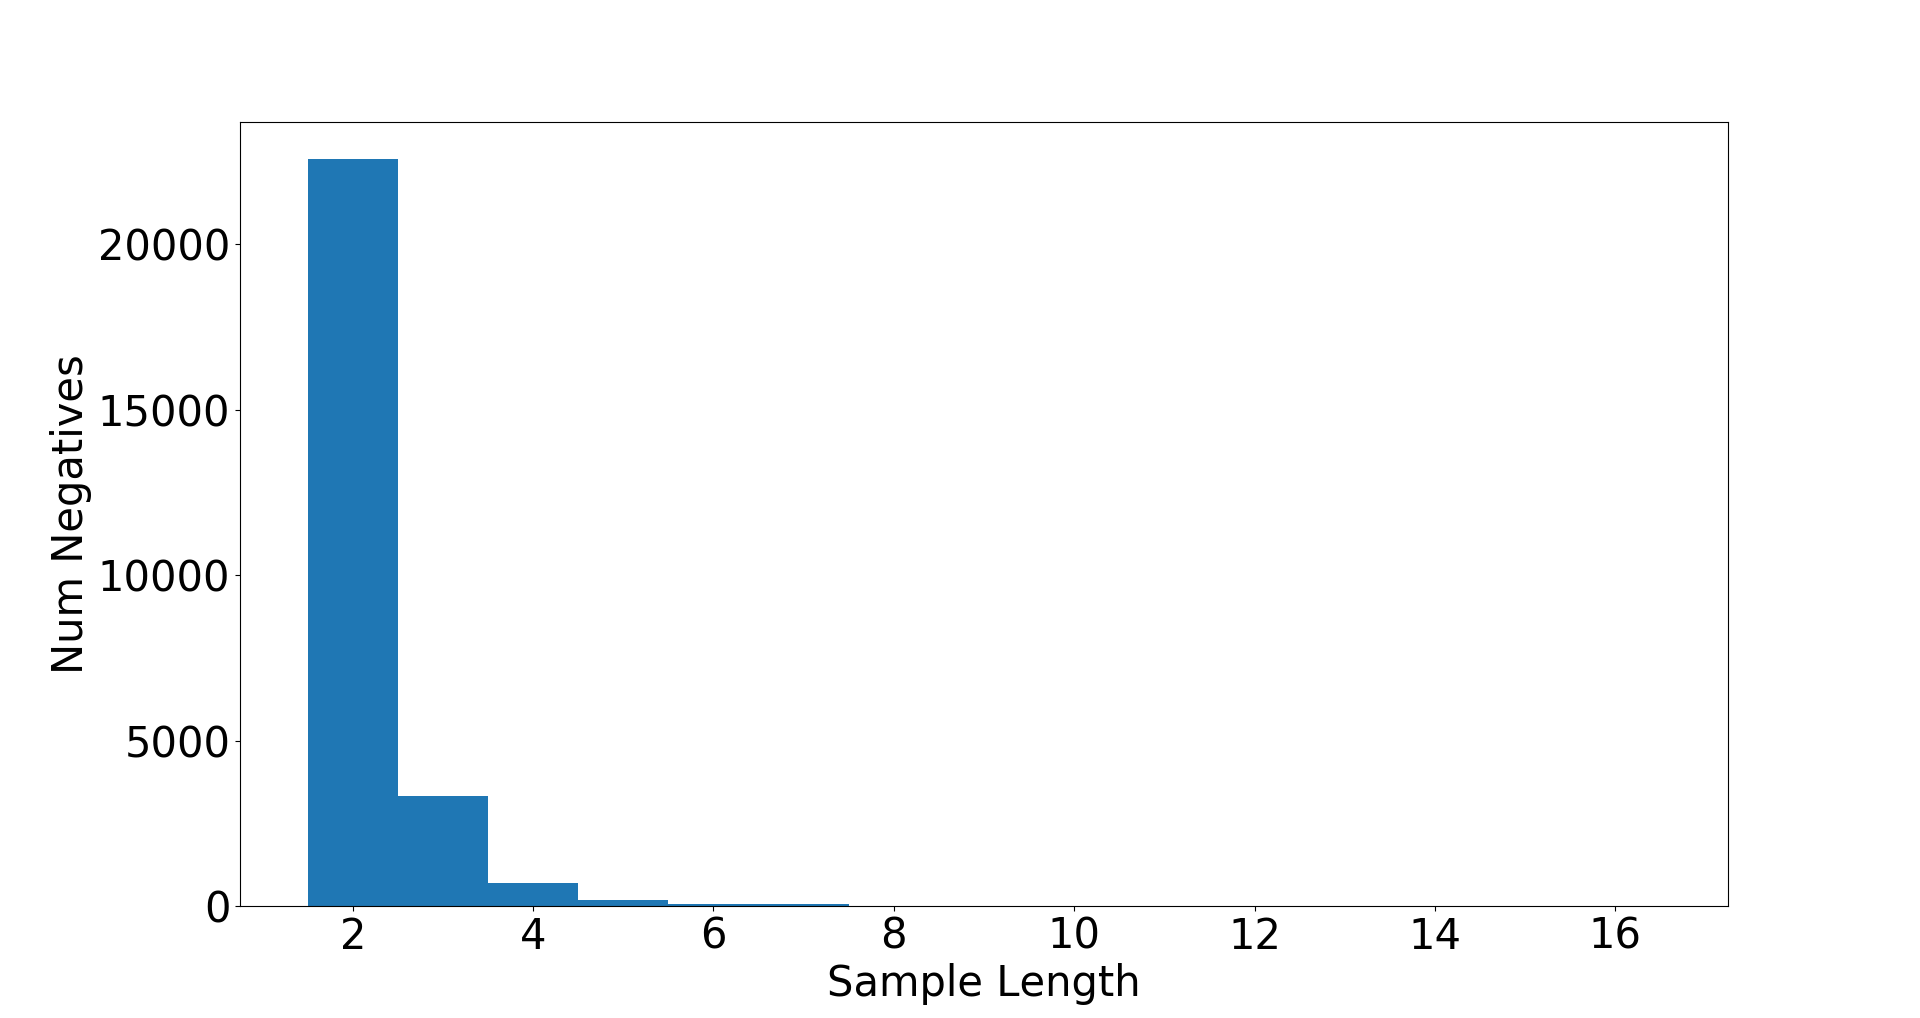
\includegraphics[width=.75\textwidth]{nSampleLenHistmin1_5max1_0Font.png}
  \caption{Distribution of pauses in the LRS3 dataset}
  \label{fig:negHist}
\end{figure}


As described earlier the LRS3 dataset is designed for visual speech recognition so it is important to analyze the dataset with respect to the usability for VVAD. Knowing the visual speech recognition background of the dataset it is quite obvious that the produced binary dataset will be very imbalanced. Figure \ref{fig:sampleDistribution} shows the theoretical distribution of positive and negative samples that can be created from the LRS3.
\begin{figure}
  \centering
  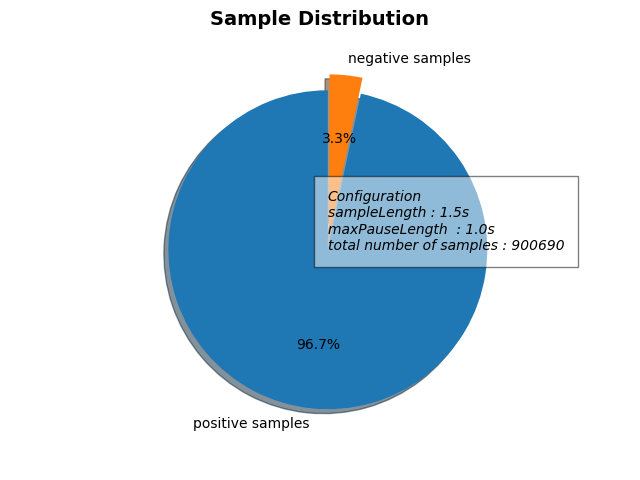
\includegraphics[width=.75\textwidth]{sampleDistribution.png}
  \caption{The theoretical distribution of positive and negative samples that can be created from the LRS3 with the given \texttt{sampleLength} and \texttt{maxPauseLength}}
  \label{fig:sampleDistribution}
\end{figure}
It shows that only 3.3\% fall in the negative class, while 96.7\% of the samples would be positive. Although that seems very little on the first look these 3.3\% are approximately 30 thousand samples, resulting in 12.5 hours of negative samples. 
For reasons of capacity it is decided to undersample the positive samples and take a positive-to-negative ratio of 1 to 1 (see section \ref{sec:problemsBigData}). 
This leads to over 60 thousand samples with an overall length of over 24 h.
In the process of creating those samples some appeared not to be valid, because the automatic conversion from the LRS3 samples to VVAD samples couldn't find a face or found to many in the corresponding LRS3 sample. 
This leads to 22,245 negative (\emph{not speaking}) samples and 22,244 positive (\emph{speaking}) samples and 18.5 h of learning data in total. 
The resulting samples are checked visually on a random basis to make sure the transformation from the LRS3 to the designated VVAD dataset is performed correctly.


With \texttt{sampleLength} and \texttt{maxPauseLength} set samples are extracted and the LRS3 dataset is transformed into a designated VVAD dataset.
At first the pauses, which later will be transformed to negative samples for the VVAD dataset, need to be extracted. 
Algorithm \ref{alg:detectPauses} shows how pauses are extracted from a LRS3 sample (an example of a LRS3 sample can be found in Appendix \ref{app:dataSample}).
Algorithm \ref{alg:detectPauses} is also used to analyze the LRS3 dataset and produce figure \ref{fig:negHist}.
From the these pauses negative and positive VVAD samples can be extracted.
Algorithm \ref{alg:getSampleConfigs} shows how the frames for the VVAD samples will be chosen from a LRS3 sample.
In section \ref{ssec:dataPreprocessing} is described how the preprocessing is performed and how the features for the VVAD sample will be extracted from a LRS3 video.

\begin{algorithm}[tbp]
\caption{}
\label{alg:detectPauses} 
\begin{algorithmic}[1]     % [1] = all lines are numbered
\Procedure{detectPauses}{$sample$}

	\Statex Returns a List of pauses in speech for a given LRS3 sample

	\algorithmicrequire{LRS3 Data Sample of speech}

	\algorithmicensure{List of Pauses}

	\State $oldWord \gets undefined$
	\State $listOfPauses \gets []$
	\State $maxPauseLength$ \Comment{defines the maximal length of a inter speech pause}

	\For{$word\ in\ sample$} \Comment{word consist of $start, end$ of the spoken word}

		\If{ $oldWord \ not \  undefined$}
		 \If{ $word.start - oldWord.end > maxPauseLength$}
				\State $listOfPauses.add((oldWord.end, word.start))$ \Comment{add pause to list}
		 \EndIf
 			\State $oldWord \gets word$

		\EndIf
		\EndFor
		
		\State \Return $listOfPauses$
\EndProcedure
\end{algorithmic}
\end{algorithm}

\begin{algorithm}[tbp]
\caption{}
\label{alg:getSampleConfigs} 
\begin{algorithmic}[1]     % [1] = all lines are numbered
\Procedure{getSampleConfigs}{$sample$}

	\Statex Returns a List of VVAD sample configs for a given LRS3 sample

	\algorithmicrequire{LRS3 Data Sample of speech}

	\algorithmicensure{List of VVAD sample configs}
	\State $sampleLength$ \Comment{defines the length of a VVAD sample}
	\State $k \gets sampleLength \times fps$ \Comment{defines the length the VVAD sample in frames}
		
	\State $listOfPauses \gets \textsc{detectPauses}(sample)$
	
	\State $negativeFrames \gets Set(listOfPauses)$ \Comment{set of frames corresponding to pauses}
	\State $sampleConfigs \gets []$
	\While{$frameNum\ in\ sample$}
		\State $nextFrames \gets Set(frameNum\ to\ frameNum + k)$
		\State $i \gets Intersection(negativeFrames, nextFrames)$ 
		\Switch{$i$}
    		\Case{$i == 0$} \Comment{It is a positive VVAD sample}
      			\State $sampleConfigs.add([True, nextFrames])$ \Comment{Add sample}
      			\State $frameNum += k$ \Comment{jump to the frame after the added sample}
    		\EndCase
		    \Case{$i == k$}\Comment{It is a negative VVAD sample}
      			\State $sampleConfigs.add([False, nextFrames])$ \Comment{Add sample}
      			\State $frameNum += k$ \Comment{jump to the frame after the added sample}
		    \EndCase
		    \Case{$0<i<k$}
		    	\State $frameNum += 1$ \Comment{just check the next k frames}
		    \EndCase
		\EndSwitch
	\EndWhile 
	
	\State \Return $sampleConfigs$

\EndProcedure
\end{algorithmic}
\end{algorithm}

\subsection{Data Preprocessing}\label{ssec:dataPreprocessing}
As described in section \ref{ssec:preprocessing} preprocessing is an elementary part of nearly every machine learning process. 
In the case of the VVAD the preprocessing handles the transformation from a video stream to VVAD samples consisting of \texttt{k} frames of features and a label. 
For every image in the stream a detected face will be followed throughout consecutive images in that stream. 
From these faces the VVAD sample will be extracted. 
The insights of how face detection and the tracking works can be found in Section \ref{ssec:faceDetection} and Section \ref{ssec:objectTracking}. 
For the End-to-End learning approach images are needed. 
These images need to be resized to a fixed size. 
To keep the original image ratio, zero padding needs to be applied in some cases.
Why a fixed image size is needed and the concept of zero padding is described in section \ref{ssec:reAndPad}.
For the facial features approach the features need to be normalized.
The preprocessing steps can also be used in live inference.


\subsubsection{Face Tracking}
To construct a VVAD sample from a LRS3 sample it is important to track a face in the video sequence, instead of only using face detection.
The approach of using only face detection can fail if multiple faces are present in the video.
To track a face dlib's correlation filter based tracker (see Section \ref{ssec:objectTracking}) is used.
On the tracked area a face detection (see Section \ref{ssec:faceDetection}) is performed to ensure correctness of the tracking and return an image of a face for every frame.
As described before the face tracking can also be used in a productive live system while making inference because inference needs to be done with samples of the same size as the training samples.


\subsubsection{Feature Generation}
To come from the tracked face to the features needed for the four different learning approaches described in Section \ref{ssec:algorithm} a \emph{Feature Generator} is implemented.
This feature generator takes a tracked image as input and outputs 
\begin{itemize}
\item[•] \textbf{Face Images -}  The whole image resized and zero padded to a specific size.
\item[•] \textbf{Lip Images -} An image of only the lips resized and zero padded to a specific size.
\item[•] \textbf{Face Features -} All 68 facial landmarks extracted with dlib's facial landmark detector
\item[•] \textbf{Lip Features -} All facial landmarks concerning the lips extracted with dlib's facial landmark detector 
\end{itemize}
For the face images the input image only needs to be resized and zero padded to a given size. Why and how this is done is described in Section \ref{ssec:reAndPad}.
For the other approaches dlib's facial landmark detector 
is used. 
As depicted in Figure \ref{fig:flavors} the predictor extracts the shape of a face given by 68 landmarks, whileas 20 of these landmarks are describing the lips.
The predictor is trained on the ibug 300-W face landmark dataset (\url{https://ibug.doc.ic.ac.uk/resources/facial-point-annotations/}). 
The iBUG 300-W face landmark dataset is provided for research purposes only. Commercial use (i.e., use in training commercial algorithms) is not allowed.
Because dlib's facial landmark detector is used to construct the VVAD dataset for lip images as well as the VVAD datasets for face and lip features, these fall under the same restrictions.
For the \emph{lip images} the minimal values in x- and y-direction are taken as the upper left corner of the lip image, while the lower right corner is defined by the maximal values in x- and y-direction.
The \emph{face features} are taken directly from the landmarks given from dlib's facial landmark detector. 
For the \emph{lip features} only landmark 49 to landmark 68 are taken into account, because they fully describe the lip shape as seen in Figure \ref{fig:shape}.
It is to mention that it is useful to normalize the features for \emph{face features} and \emph{lip features} when applied to a learning algorithm. 
The used normalization is described in Section \ref{ssec:normalize}.

\begin{figure}
  \centering
  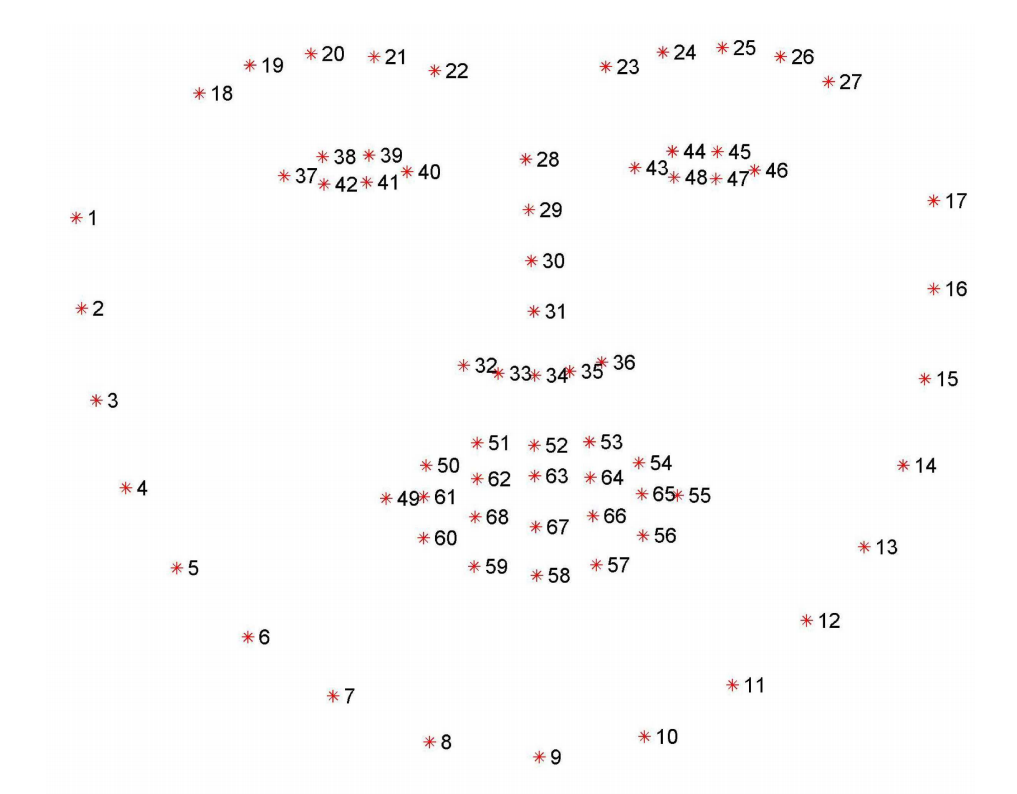
\includegraphics[width=.75\textwidth]{shape.png}
  \caption{The annotations given for the ibug 300-W dataset \cite{6755925}}
  \label{fig:shape}
\end{figure}

As well as the face tracking the generator can also be used in a live inference system to generate the features needed for the corresponding algorithm.


\subsubsection{Resize and Padding}\label{ssec:reAndPad}
Theoretically neural networks can work on images of different sizes, just like humans can detect a specific object even if they are only looking through a very small hole.
The limitations in artificial neural networks are computational.
Keras works with NumPy arrays as input. These are multidimensional arrays with fixed dimensions.
If gradient descent should be carried out with mini batches or the whole dataset the array will have a shape of $(DS \times SD)$ or $(BS \times SD)$ respectively, where $DS$ is the size of the whole dataset and $BS$ is the batch size, while $SD$ are the sample dimensions. The array for one batch of VVAD samples with the batch size 64 would have a shape of $(64 \times 38 \times 200 \times 200 \times 3)$ if face images would be considered and $(64 \times 38 \times 68)$ if face features would be considered.
The resizing is needed to produce a constant input size for the model but faces do not always have the same ratio and therefore the bounding boxes from the face detection do neither.
It is in fact important to keep the ratio of the face steady over all timesteps to reduce distortion over time which could be interpreted as mouth movement.
If a specific size is needed but it can't be fulfilled zero padding is a common technique to tackle this problem.
Zero padding just inputs zero values where no information can be provided. The NN will learn that zero means \emph{no information}.
For the resizing of face images this means that the face image is resized to the maximal size which would fit into the goal size and all pixels that can't be used on the right or lower site will be filled with zeros.




\subsection{Testing human Accuracy Level on the VVAD Dataset}\label{ssec:VVADHACL}
To test the VVAD dataset a human accuracy test was performed.
The test used a randomly seeded subset of 200 samples and was performed on 10 persons.
The overall human accuracy level was 87.93\% while the human accuracy level on positive samples is 91.44\% the human accuracy level on negative samples is only 84.44\%.
This shows, that the automatic extraction of the negative samples is more prone to errors than the automatic extraction of positive samples. This is due to the purpose of the LRS3 as a lipreading dataset which obviously offers more positive samples than negative samples for a VVAD dataset. 

\begin{figure}
  \centering
  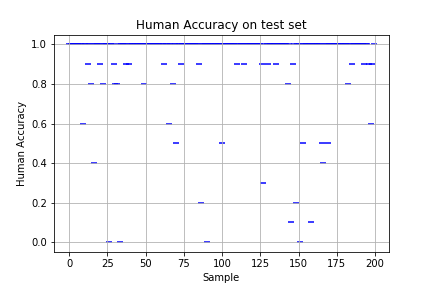
\includegraphics[width=.75\textwidth]{humanAcc.png}
  \caption{The human accuracy for each sample}
  \label{fig:humanAcc}
\end{figure}

\begin{figure}
  \centering
  \includegraphics[width=.75\textwidth]{PosHumanAcc.png}
  \caption{The human accuracy for each sample in the positive class}
  \label{fig:PosHumanAcc}
\end{figure}

\begin{figure}
  \centering
  \includegraphics[width=.75\textwidth]{NegHumanAcc.png}
  \caption{The human accuracy for each sample in the negative class}
  \label{fig:NegHumanAcc}
\end{figure}

In Figure \ref{fig:humanAcc} the accuracy for the individual samples is shown. Figure \ref{fig:PosHumanAcc} and \ref{fig:NegHumanAcc} show the human accuracy levels of each sample for the two classes.
It shows that a lot of the samples are classified with a very high accuracy, while some are obviously labeled wrong because they have a very high wrong classification rate. For the given reason these wrong labels appear more often in the negative class.
These wrongly labeled samples in the validation set make it hard to get a very high accuracy in the validation while tuning the learning algorithm.
But it is important to know this border, to tune to a value close to that.
If these wrongly labeled samples are not present in the test set, the accuracy of the final test can be higher. 
This shows how the learning algorithm can be robust against these outliers in the learning process. 

The test was implemented as a Web App using Node.js\cite{NODE} with Express\cite{EXPRESS} and a mongoDB\cite{MONGO} in the Back-End and HTML5 in the Front-End.
It shows a simple self explanatory graphical user interface which displays a video sequence of a \emph{speaking} or \emph{not speaking} person and three buttons (see figure \ref{fig:gui}). 
With the buttons it is possible to classify the sample as either \emph{speaking} or \emph{not speaking} and to repeat the video sequence.

\begin{figure}
  \centering
  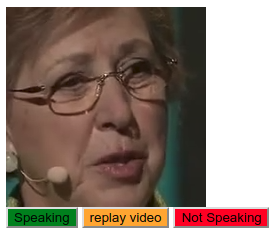
\includegraphics[width=.75\textwidth]{gui.png}
  \caption{The graphical user interface for the human accuracy test}
  \label{fig:gui}
\end{figure}



\section{Implementations of the Learning Algorithms}\label{sec:implLearning}
As stated in Section \ref{ssec:algorithm} LSTM-FCNs are state of the art in classification for video sequences and LSTMs in general work really well for time series.
To implement these Deep Learning techniques Keras is used.
Keras makes it possible to go very fast from a design to a prototype which makes it very valuable for research.
Following two End-to-End learning approaches and two approaches using manually extracted facial features will be presented.

End-to-End Learning describes a learning approach where raw data is feed to an ANN and the ANN is deep enough to learn all important features itself. For the example of a VVAD the ANN would be able to learn, that it makes sense to look for the mouth to see if a person is peaking or not.
In contrast in Section \ref{ssec:facialFeaturesLearninig} the important features are manually extracted before.
This approach needs more domain knowledge about the problem but can result in a substantially smaller model.
It is a common practice to start with the biggest possible model to get reasonable results to subsequently make the model small while trying to sustain accuracy.


\subsection{End-to-End Learning}\label{ssec:EndToEndLearning} %Maybe just one Chapter for End-to-End
To implement a End-to-End Learning Algorithm the following five Models  were taken to evaluate a Baseline:

\begin{itemize}
\item DenseNet201
\item DenseNet121
\item MobileNet
\item MobileNetV2
\item VGGFace
\end{itemize}

Where the first four Models are taken from the Keras Applications (\url{https://keras.io/applications/}), while the VGGFace is a taken from \url{https://github.com/rcmalli/keras-vggface}. 
DenseNet and MobileNet are more general models for image classification, that perform well on the ImageNet dataset \cite{imagenet_cvpr09}, whereas VGGFace was chosen because it is implemented explicitly for faces.
The Baseline Accuracy is taken from theses models applied on only the first image of every sample in the VVAD dataset.
Figure \ref{fig:baseAccDense201} to \ref{fig:baseAccVGGFace} show the accuracy for 200 epochs.
With this approach a Baseline Accuracy between 67.45\% for MobileNetV2 and 73.17\% for DenseNet121 can be reached.

\begin{figure}
  \centering
  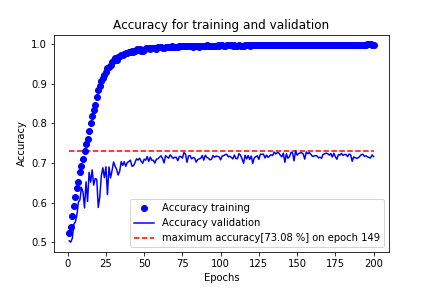
\includegraphics[width=.75\textwidth]{FINALBASELINEDenseNet_64_(96,96,3)_2019-08-0721:58:16029339_accuracy.png}
  \caption{Baseline Accuracy for DenseNet201}
  \label{fig:baseAccDense201}
\end{figure}

%\begin{figure}
%  \centering
%  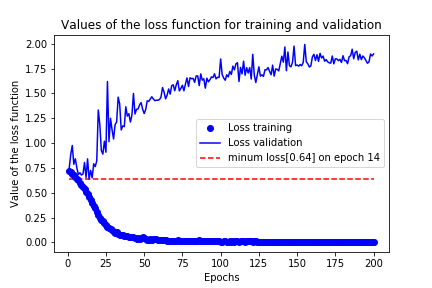
\includegraphics[width=.75\textwidth]{FINALBASELINEDenseNet_64_(96,96,3)_2019-08-0721:58:16029339_loss.png}
%  \caption{Baseline Loss for DenseNet201}
%  \label{fig:baseLossDense201}
%\end{figure}

%------------------------------

\begin{figure}
  \centering
  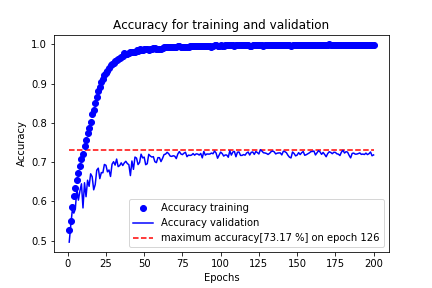
\includegraphics[width=.75\textwidth]{FINALBASELINEDenseNetSmall_64_(96,96,3)_2019-08-0817:39:46410269_accuracy.png}
  \caption{Baseline Accuracy for DenseNet121}
  \label{fig:baseAccDense121}
\end{figure}

%\begin{figure}
%  \centering
%  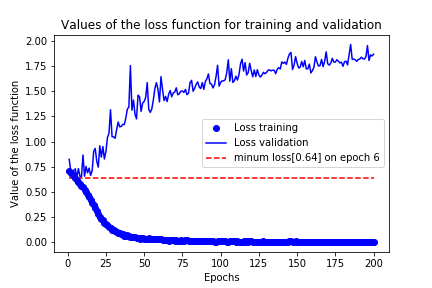
\includegraphics[width=.75\textwidth]{FINALBASELINEDenseNetSmall_64_(96,96,3)_2019-08-0817:39:46410269_loss.png}
%  \caption{Baseline Loss for DenseNet121}
%  \label{fig:baseLossDense121}
%\end{figure}

%%------------------------------

\begin{figure}
  \centering
  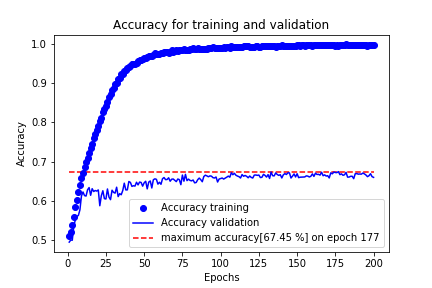
\includegraphics[width=.75\textwidth]{FINALBASELINEMobileNet_64_(96,96,3)_2019-08-0713:47:03006586_accuracy.png}
  \caption{Baseline Accuracy for MobileNetV2}
  \label{fig:baseAccMobile2}
\end{figure}

%\begin{figure}
%  \centering
%  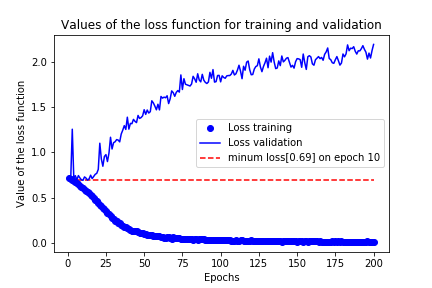
\includegraphics[width=.75\textwidth]{FINALBASELINEMobileNet_64_(96,96,3)_2019-08-0713:47:03006586_loss.png}
%  \caption{Baseline Loss for MobileNetV2}
%  \label{fig:baseLossMobile2}
%\end{figure}

%%------------------------------
%
\begin{figure}
  \centering
  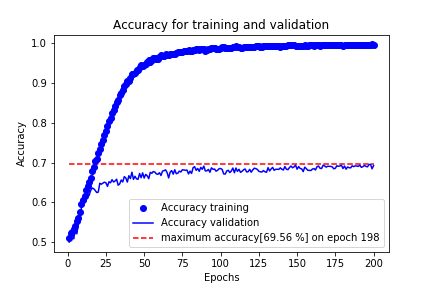
\includegraphics[width=.75\textwidth]{FINALBASELINEMobileNetV1_64_(96,96,3)_2019-08-0812:27:51418544_accuracy.png}
  \caption{Baseline Accuracy for MobileNetV1}
  \label{fig:baseAccMobile1}
\end{figure}

%\begin{figure}
%  \centering
%  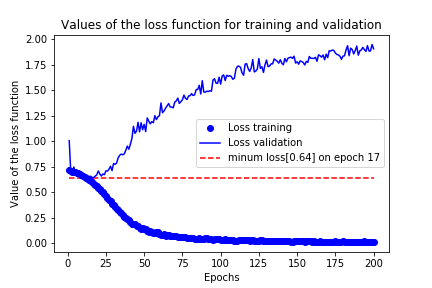
\includegraphics[width=.75\textwidth]{FINALBASELINEMobileNetV1_64_(96,96,3)_2019-08-0812:27:51418544_loss.png}
%  \caption{Baseline Loss for MobileNetV1}
%  \label{fig:baseLossMobile1}
%\end{figure}
%
%%------------------------------

\begin{figure}
  \centering
  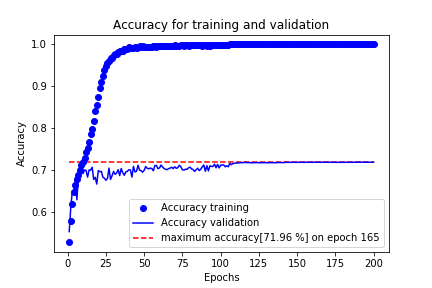
\includegraphics[width=.75\textwidth]{FINALBASELINEVGGFace_64_(96,96,3)_2019-08-0803:01:24022816_accuracy.png}
  \caption{Baseline Accuracy for VGGFace}
  \label{fig:baseAccVGGFace}
\end{figure}

%\begin{figure}
%  \centering
%  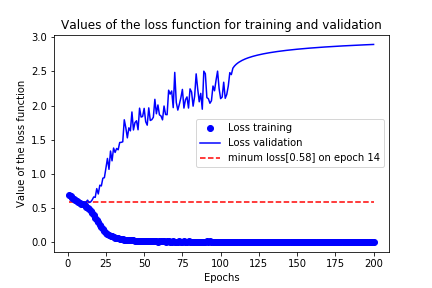
\includegraphics[width=.75\textwidth]{FINALBASELINEVGGFace_64_(96,96,3)_2019-08-0803:01:24022816_loss.png}
%  \caption{Baseline Loss for VGGFace}
%  \label{fig:baseLossVGGFace}
%\end{figure}

%------------------------------

The Baseline Models make spatial sense out of the images by producing meaningful features, which can be used to classify a single image.
This relies mostly on a combination of Convolutional Layers, as described in Section \ref{ssec:Conv}.
The optimal image size is evaluated for the MobileNet using quadratic image sizes starting from $32 \times 32$ to the maximal image size of $200 \time 200$ with a step size of 32.
Figure \ref{fig:AccOverImagesize} shows that the maximal accuracy in the spatial domain can be reached using a image size of $160 \times 160$.
\begin{figure}
  \centering
  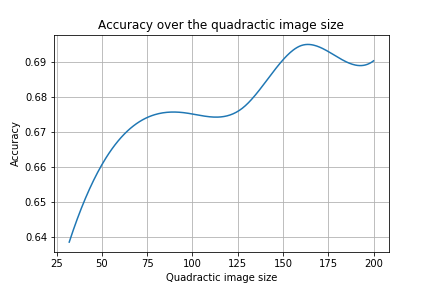
\includegraphics[width=.75\textwidth]{AccOverImagesize.png}
  \caption{Evaluation of the optimal image size}
  \label{fig:AccOverImagesize}
\end{figure}


As described earlier speech can't be classified effectively by only one image, that's why the baseline accuracy levels around 70\% depending o the model.
To enhance these results a temporal sense must be extracted from a series of images.
To do so LSTM cells, as described in Section \ref{ssec:LSTM}, are used.
The overall model structure can be seen in Figure \ref{fig:model}.

\begin{figure}
  \centering
  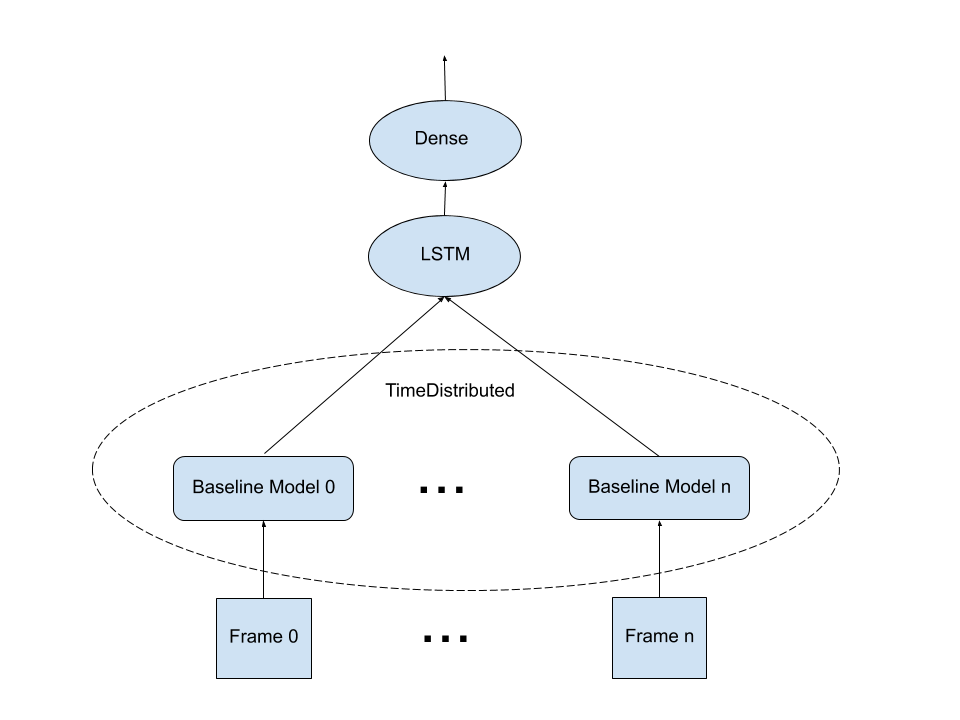
\includegraphics[width=.75\textwidth]{modelStructure.png}
  \caption{Model structure using a \emph{TimeDistributed} Baseline Model}
  \label{fig:model}
\end{figure}

Here it can be seen, that a \emph{TimeDistributed} wrapper was used.
\emph{TimeDistributed} is a wrapper provided by Keras which basically copies a model for all timesteps, to effectively handle time series.
This allows the Baseline Models to be used to produce a time series from the features of all frames. 
The time series can be used by the LSTM Layer to make temporal sense, while the last Dense Layer is used to make the classification.
Experiments have shown that a single Dense layer with 512 units on top of a LSTM layer with 32 units show decent results.
To evaluate the increase in accuracy DenseNet121, MobileNet and VGGFace are used as base models in the \emph{TimeDistributed} wrapper and instead of only one image the first two images are taken in consideration.
Figure \ref{fig:tD2Dense} to \ref{fig:tD2VGGFace} show that DenseNet121, MobileNet and VGGFace improve by around 2.3\% with one more timestep.

\begin{figure}
  \centering
  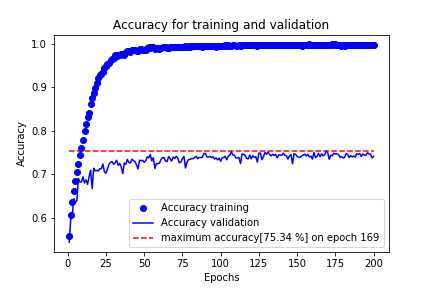
\includegraphics[width=.75\textwidth]{all_TimeDistributedDenseNet_1_32_1_512_64_(2,96,96,3)_2019-08-1308:08:20668409_accuracy.png}
  \caption{Accuracy for a \emph{TimeDistributed} DenseNet121 on two timesteps}
  \label{fig:tD2Dense}
\end{figure}

\begin{figure}
  \centering
  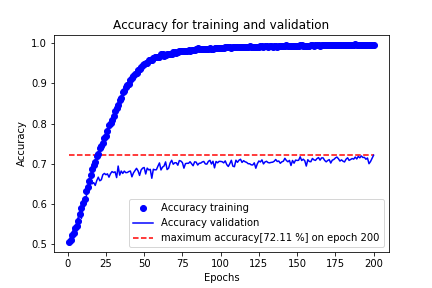
\includegraphics[width=.75\textwidth]{all_TimeDistributedMobileNet_1_32_1_512_64_(2,96,96,3)_2019-08-1217:56:08538419_accuracy.png}
  \caption{Accuracy for a \emph{TimeDistributed} MobileNet on two timesteps}
  \label{fig:tD2Mobile}
\end{figure}

\begin{figure}
  \centering
  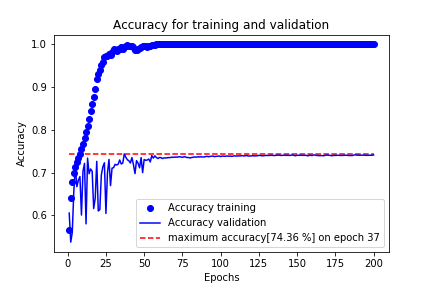
\includegraphics[width=.75\textwidth]{all_TimeDistributedVGGFace_1_32_1_512_64_(2,96,96,3)_2019-08-1316:53:40647699_accuracy.png}
  \caption{Accuracy for a \emph{TimeDistributed} VGGFace on two timesteps}
  \label{fig:tD2VGGFace}
\end{figure}

For more timesteps it can be seen in Figure \ref{fig:model} that the base model will be copied for every new timestep which results in a very fast growth of the model which can cause that the model is not trainable on modern Hardware.
To prevent that only the MobileNet as the smallest of the base models is taken further into consideration.
In comparison MobileNet trains approximately 4,2 million parameters while DenseNet trains around double the amount with 8 million parameters and VGGFace trains over 50 million parameters.
Knowing this the MobileNet is a good compromise between performance and size, because it is able to consider more timesteps, which in the end can lead to even higher accuracy.
The \emph{TimeDistributed} MobileNet with four timesteps already reaches a higher accuracy. Figure \ref{fig:AccTimeStepsMobile} shows how the accuracy raises over the number of used frames for the \emph{timeDistributred} MobileNet.

\begin{figure}
  \centering
  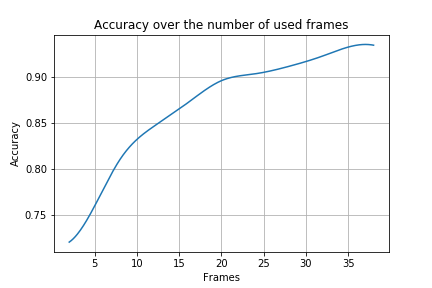
\includegraphics[width=.75\textwidth]{AccOverFrames.png}
  \caption{Validation Accuracy for the \emph{TimeDistributed} MobileNet over the number of timesteps/frames used.}
  \label{fig:AccTimeStepsMobile}
\end{figure}

Taking Figure \ref{fig:AccTimeStepsMobile} and \ref{fig:AccOverImagesize} into account the optimal values for the image size and number of frames are $160 \times 160$ and 36 respectively.
This model couldn't be trained on modern GPUs because it was to big for the internal memory. 
Since the image size has a quadratic influence on the memory consumption a image size of $96 \times 96$ was taken instead to make the training possible.
For the training of the model 15\% of the data is taken as validation data.
Figure \ref{fig:FaceEndToEndHistory} shows how the validation accuracy evolves over the training episodes.

\begin{figure}
  \centering
  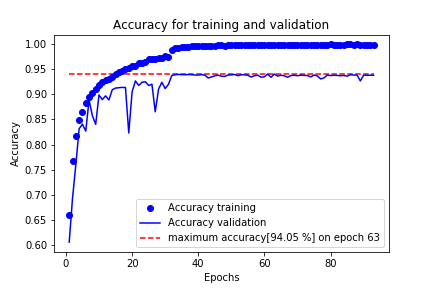
\includegraphics[width=.75\textwidth]{FaceEndToEndHistory.png}
  \caption{The End-To-End Learning approach using Face Images reaches a Validation Accuracy of 94.05\%.}
  \label{fig:FaceEndToEndHistory}
\end{figure}

As described in Section \ref{ssec:VVADHACL} the overall human accuracy level is only 87.93\%.
The result of the End-To-End Learning approach on Face Images need to be evaluated on the test set, but the validation accuracy is a strong indicator that the produced model performs can reach \emph{superhuman performance}, which means it performs better than a human could do on the same task.

The same architecture is applied to the \emph{Lip Images} flavor of the VVAD dataset.
Here the domain knowledge about speech is applied as the assumption that the recognition of speech is only depending on the lips.
The results of the training are depicted in Figure \ref{fig:LipEndToEndHistory}.

\begin{figure}
  \centering
  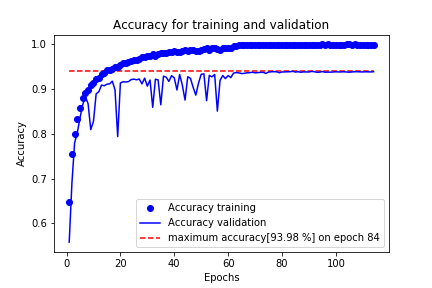
\includegraphics[width=.75\textwidth]{LipEndToEndHistory.png}
  \caption{The End-To-End Learning approach using Lip Images reaches a Validation Accuracy of 93.98\%.}
  \label{fig:LipEndToEndHistory}
\end{figure}
As the validation accuracy went from 94.05\% for the Face Images only to 93.98\% for the Lip Images the assumption can be viewed as true. 
Taking only the Lip Images with the full resolution already reduces the amount of data needed to be kept in the GPU's RAM by approximately the half because the image size as the driving factor was reduced by half.
Also the trained model can be reduced in size from 35.6 MB to 29.3 MB.
These results need to be evaluated on the test set as well as the results of the approach using face images.

\subsection{Learning on Facial Features}\label{ssec:facialFeaturesLearninig} %Maybe just one Chapter for Facial Features
As described in Section \ref{sec:vvadData} the VVAD dataset also provides a version of the dataset which already exposes only facial landmarks.
In the End-To-End Learning approach features where produced from the images using MobileNet as a base model which was \emph{TimeDistributed} over k frames.
The resulting spatial features where forwarded to a LSTM layer to make temporal sense.
Since the \emph{face features} and \emph{lip features} flavor have already extracted spatial features it is no longer necessary to use a \emph{TimeDistributed} base model.
The facial landmarks are normalized as depicted in Section \ref{ssec:normalize} and then used by the head of the architecture used for the End-To-End Learning approach, which is a single LSTM layer with 32 units and a single Dense layer with 512 units.
Figure \ref{fig:FaceFeaturesHistory} shows that even with the substantially smaller dataset of the face features a validation accuracy of 89.79\% can be reached which is still higher than the human accuracy level.

\begin{figure}
  \centering
  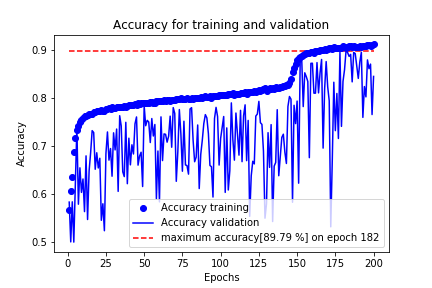
\includegraphics[width=.75\textwidth]{FaceFeaturesHistory.png}
  \caption{The Facial Features for Learning approach using all 68 facial landmarks reaches a Validation Accuracy of 89.79\%.}
  \label{fig:FaceFeaturesHistory}
\end{figure}
The model size for this approach is approximately 100 times smaller with 342.5 KB.
But it is also visible that the validation accuracy is very unstable which is an indicator that it will not generalize as good as the prior models.
The essentially smaller model size can be a good compromise for weaker systems to perform the predictions to still get reasonable results.
An even smaller model can be trained with the lip features flavor of the VVAD dataset.
For this approach the same architecture as for the face features is used.
In Figure \ref{fig:LipFeaturesHistory} the validation accuracy over the epochs is displayed for the learning approach using only the 20 facial landmarks corresponding to the lips.

\begin{figure}
  \centering
  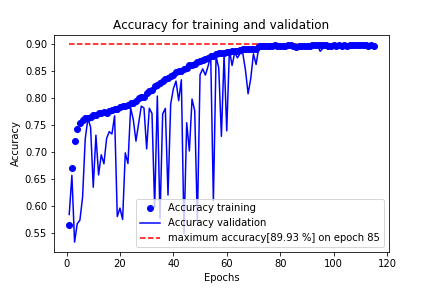
\includegraphics[width=.75\textwidth]{LipFeaturesHistory.png}
  \caption{The Facial Features for Learning approach using the 20 facial landmarks corresponding to the lips reaches a Validation Accuracy of 89.93\%.}
  \label{fig:LipFeaturesHistory}
\end{figure}

Here the accuracy is slightly better than the accuracy for using all 68 facial landmarks. 
This shows that the approach with all facial landmarks could probably be tuned a little more, but since the smaller model already shows higher accuracy it can be viewed as the tuned version of the approach using all facial landmarks.
Which also can be seen here is that the instability in the validation accuracy can be reduced.
This results need to be evaluated on the test set but the results for the validation accuracy are very promising that even for weaker hardware reliable predictions can be made.

\subsubsection{Feature Normalization}\label{ssec:normalize}
As described in Section \ref{ssec:normalization} normalizing features is a very helpful step to make NN more efficient.
Algorithm \ref{alg:normalize} describes how the facial landmarks extracted from dlib's facial landmark detector
are normalized.

\begin{algorithm}[tbp]
\caption{}
\label{alg:normalize} 
\begin{algorithmic}[1]     % [1] = all lines are numbered
\Procedure{calcDistances}{$sample$}

	\Statex Returns a List of euclidean distances to the first landmark in the sample
	
	\algorithmicrequire{List of facial landmarks }

	\algorithmicensure{List of euclidean distances}

	\State $base \gets sample[0][0]$
	\State $dists \gets []$
	\State $normalizedLandmarks \gets normalize(distances)$
	
	\For{$frame\ in\ sample$} 
		\State $distFrame \gets []$
		\For{$landmark\ in\ frame$} 
			\State $distPoint \gets []$
			\State $distPoint[0] = landmark[0] - base[0]$
			\State $distPoint[1] = landmark[1] - base[1]$
			\State $distFrame.append(distPoint)$
		\EndFor
		\State $dists.append(distFrame)$
	\EndFor
		\State \Return $dists$
\EndProcedure

\Procedure{normalize}{$distances$}

	\Statex Returns a List of normalized euclidean distances
	
	\algorithmicrequire{List of euclidean distances}

	\algorithmicensure{List of normalized euclidean distances}

	\State $absMax \gets max(abs(distances))$
	\State $normalizedDistances \gets []$
	\For{$frame\ in\ distances$} 
		\For{$dist in frame$}		
			\State $normalizedDist \gets dist / absMax$
			\State $normalizedDistances.append(normalizedDist)$
		\EndFor
	\EndFor
	
		\State \Return $normalizedDistances$
\EndProcedure

\Procedure{normalizeFacialLandmarks}{$landmarks$}

	\Statex Returns a List of normalized facial landmarks
	
	\algorithmicrequire{List of facial landmarks }

	\algorithmicensure{List of normalized facial landmarks}

	\State $distances \gets calcDistances(landmarks)$
	\State $normalizedLandmarks \gets normalize(distances)$
	
		\State \Return $normalizedLandmarks$
\EndProcedure
\end{algorithmic}
\end{algorithm}
